\documentclass[12pt]{article}

%% The graphicx package provides the includegraphics command.
\usepackage{graphicx}
%% The amssymb package provides various useful mathematical symbols
\usepackage{amssymb}
%% The amsthm package provides extended theorem environments
%% \usepackage{amsthm}
\usepackage{amsmath}
\usepackage{listings}
% \usepackage{epstopdf}

%% The lineno packages adds line numbers. Start line numbering with
%% \begin{linenumbers}, end it with \end{linenumbers}. Or switch it on
%% for the whole article with \linenumbers after \end{frontmatter}.
% \usepackage{lineno}

%% natbib.sty is loaded by default. However, natbib options can be
%% provided with \biboptions{...} command. Following options are
%% valid:

%%   round  -  round parentheses are used (default)
%%   square -  square brackets are used   [option]
%%   curly  -  curly braces are used      {option}
%%   angle  -  angle brackets are used    <option>
%%   semicolon  -  multiple citations separated by semi-colon
%%   colon  - same as semicolon, an earlier confusion
%%   comma  -  separated by comma
%%   numbers-  selects numerical citations
%%   super  -  numerical citations as superscripts
%%   sort   -  sorts multiple citations according to order in ref. list
%%   sort&compress   -  like sort, but also compresses numerical citations
%%   compress - compresses without sorting
%%
%% \biboptions{comma,round}

% \biboptions{}

\begin{document}

%% Title, authors and addresses

\title{1-D Simulation of Western Boundary Current}

%% use the tnoteref command within \title for footnotes;
%% use the tnotetext command for the associated footnote;
%% use the fnref command within \author or \address for footnotes;
%% use the fntext command for the associated footnote;
%% use the corref command within \author for corresponding author footnotes;
%% use the cortext command for the associated footnote;
%% use the ead command for the email address,
%% and the form \ead[url] for the home page:
%%
%% \title{Title\tnoteref{label1}}
%% \tnotetext[label1]{}
%% \author{Name\corref{cor1}\fnref{label2}}
%% \ead{email address}
%% \ead[url]{home page}
%% \fntext[label2]{}
%% \cortext[cor1]{}
%% \address{Address\fnref{label3}}
%% \fntext[label3]{}

\author{Chuning Wang}

% \begin{abstract}
% %% Text of abstract
% Suspendisse potenti. Suspendisse quis sem elit, et mattis nisl. Phasellus consequat erat eu velit rhoncus non pharetra neque auctor. Phasellus eu lacus quam. Ut ipsum dolor, euismod aliquam congue sed, lobortis et orci. Mauris eget velit id arcu ultricies auctor in eget dolor. Pellentesque suscipit adipiscing sem, imperdiet laoreet dolor elementum ut. Mauris condimentum est sed velit lacinia placerat. Vestibulum ante ipsum primis in faucibus orci luctus et ultrices posuere cubilia Curae; Nullam diam metus, pharetra vitae euismod sed, placerat ultrices eros. Aliquam tincidunt dapibus venenatis. In interdum tellus nec justo accumsan aliquam. Nulla sit amet massa augue.
% \end{abstract}

% \begin{keyword}
% Science \sep Publication \sep Complicated
% %% keywords here, in the form: keyword \sep keyword
% 
% %% MSC codes here, in the form: \MSC code \sep code
% %% or \MSC[2008] code \sep code (2000 is the default)
% 
% \end{keyword}

\maketitle

%% main text
\section{Model setup}
\label{sec:setup}
\subsection{Vorticity equation}

The numerical model in this report aims to solve the 1-D vorticity equation

\begin{equation}
\frac{\partial}{\partial t}\phi_{xx} + \beta\phi_x = WC - \gamma\phi_{xx}
\label{eq:vort}
\end{equation}
 
where $\phi$ is the stream function, the terms on the left side are the 'storage term' and `$\beta$ effect term', while terms on the right side are wind curl and friction, respectively. To solve this equation numerically, the domain is set to a 1-D grid consists of $X+1$ points, and the spatial derivation terms must be discretized with finite difference method:

\begin{equation}
(\phi_x)_i^n = \frac{\phi_{i+1}^n-\phi_{i-1}^n}{2\Delta x}
\label{eq:ddx}
\end{equation}

\begin{equation}
(\phi_{xx})_i^n = \frac{\phi_{i+1}^n-2\phi_i^n+\phi_{i-1}^n}{\Delta x^2}
\label{eq:ddxx}
\end{equation}

and temporal derivation can be discretized with either forward scheme

\begin{equation}
\frac{\partial}{\partial t}(\phi_{xx})_i = \frac{(\phi_{xx})_i^{n+1}-(\phi_{xx})_i^n}{\Delta t}
\label{eq:ddtforw}
\end{equation}

or leap frog scheme

\begin{equation}
\frac{\partial}{\partial t}(\phi_{xx})_i = \frac{(\phi_{xx})_i^{n+1}-(\phi_{xx})_i^{n-1}}{2\Delta t}
\label{eq:ddtlfrog}
\end{equation}

The superscript $n$ and subscript $i$ are indices for time steps and spatial grid points, respectively. Substitute Eq~\ref{eq:ddtforw} into Eq~\ref{eq:vort} and rearrange terms

\begin{equation}
(\phi_{xx})_i^{n+1} = (\phi_{xx})_i^n + \Delta t(-\beta(\phi_x)_i^n + WC - \gamma(\phi_{xx})_i^n)
\label{eq:vortdes}
\end{equation}

then substitute Eq~\ref{eq:ddxx} into Eq~\ref{eq:vortdes} for time step $n+1$, the forward scheme, discretized 1-D vorticity equation becomes

\begin{equation}
\phi_{i+1}^{n+1}-2\phi_i^{n+1}+\phi_{i-1}^{n+1} = \Delta x^2(\phi_{xx})_i^n + \Delta x^2\Delta t(-\beta(\phi_x)_i^n + WC - \gamma(\phi_{xx})_i^n)
\label{eq:vortdes2}
\end{equation}

or using leap frog scheme

\begin{equation}
\phi_{i+1}^{n+1}-2\phi_i^{n+1}+\phi_{i-1}^{n+1} = \Delta x^2(\phi_{xx})_i^{n-1} + 2\Delta x^2\Delta t(-\beta(\phi_x)_i^n + WC - \gamma(\phi_{xx})_i^n)
\label{eq:vortdes3}
\end{equation}

For a 1-D grid consists of $X+1$ points, Eq~\ref{eq:vortdes2} and~\ref{eq:vortdes3} satisfy everywhere except at boundaries $i=0$ or $i=X$.\\

\subsection{Boundary condition}
To close the system and complete the linear equations, boundary condition are required. For this particular exercise, we use two sets of boundary conditions: first of which is `no net transport'

\begin{equation}
\phi=0~~@~~x = 0,~1
\label{eq:bc1}
\end{equation}

and second is for velocity $v$ at each boundary, which is chosen from either non-slip

\begin{equation}
\phi_x=0~~@~~x = 0,~1
\label{eq:bc2}
\end{equation}

or free-slip

\begin{equation}
\phi_{xx}=0~~@~~x = 0,~1
\label{eq:bc3}
\end{equation}

Discretizing Eq~\ref{eq:bc1}, \ref{eq:bc2} and \ref{eq:bc3} for time step $n+1$ gives

\begin{equation}
\phi_0^{n+1}=0,~\phi_X^{n+1}=0
\label{eq:bcdes}
\end{equation}

\begin{equation}
\phi_{-1}^{n+1}-\phi_{1}^{n+1}=0,~\phi_{X-1}^{n+1}-\phi_{X+1}^{n+1}=0
\label{eq:bcdes2}
\end{equation}

\begin{equation}
\phi_{-1}^{n+1}-2\phi_{0}^{n+1}+\phi_{1}^{n+1}=0,~\phi_{X-1}^{n+1}-2\phi_{X}^{n+1}+\phi_{X+1}^{n+1}=0
\label{eq:bcdes3}
\end{equation}

where $i=-1$ and $i=X+1$ are two imaginary grid points brought into the system to satisfy the second set of boundary condition.\\

\subsection{Matrix construction}
At this point, we have constructed a linear equation system with $X+3$ equations and $X+3$ unknowns. It can be expressed with a matrix form

\begin{equation}
A\phi^{n+1}=B
\end{equation}

where $A$ is a sparse matrix dependent on the choice of the second boundary condition and $B$ is a 1-D array dependent on the choice of temporal discretization scheme. An example of $A$ with non-slip condition is

\begin{equation}
A=\begin{bmatrix} 
			1 & 0 & -1 & & & & & & \\
			0 & 1 & 0 & & & & & & \\
			   &1 & -2 & 1 & & & & & \\
			   & & 1 & -2 & 1 & & & & \\
			   & & & \ddots & \ddots & \ddots & & & \\ 
			   & & & & 1 & -2 & 1 & & \\
			   & & & & & 1 & -2 & 1 & \\
			   & & & & & & 0 & 1 & 0 \\
			   & & & & & & 1 & 0 & -1 \\
	\end{bmatrix}
\label{eq:matrix}
\end{equation}

and $B$ with forward scheme is

\begin{equation}
B=\begin{bmatrix}
	0 \\
	0 \\
	\Delta x^2(\phi_{xx})_1^n + \Delta x^2\Delta t(-\beta(\phi_x)_1^n + WC - \gamma(\phi_{xx})_1^n)\\
	\Delta x^2(\phi_{xx})_2^n + \Delta x^2\Delta t(-\beta(\phi_x)_2^n + WC - \gamma(\phi_{xx})_2^n)\\
	\vdots \\
	\Delta x^2(\phi_{xx})_{X-1}^n + \Delta x^2\Delta t(-\beta(\phi_x)_{X-1}^n + WC - \gamma(\phi_{xx})_{X-1}^n)\\
	\Delta x^2(\phi_{xx})_{X-2}^n + \Delta x^2\Delta t(-\beta(\phi_x)_{X-2}^n + WC - \gamma(\phi_{xx})_{X-2}^n)\\
	0 \\
	0 \\
	\end{bmatrix}
\end{equation}

The unknown $\phi^{n+1}$ is also a 1-D array

\begin{equation}
\phi^{n+1}=\begin{bmatrix}
	\phi_{-1}^{n+1} \\
	\phi_{0}^{n+1} \\
	\phi_{1}^{n+1} \\
	\phi_{2}^{n+1} \\
	\vdots \\
	\phi_{X-2}^{n+1} \\
	\phi_{X-1}^{n+1} \\
	\phi_{X}^{n+1} \\
	\phi_{X+1}^{n+1} \\
	\end{bmatrix}
\end{equation}

Iteratively solve Eq~\ref{eq:matrix} for $n=n+1$ to move forward in temporal domain. Update velocity $v=\phi_x$ and vorticity $\zeta=\phi_{xx}$ for each step and store the solution.\\

\subsection{Numerical tips}
\begin{itemize}
\item When $N$ is a very large number, matrix $A$ becomes larger accordingly and solving the system eats up a lot of memory. However, since $A$ is a sparse matrix, Python and MATLAB both offer special algorithms to solve the equation system much more efficiently. Make sure to use these algorithms and save some time.
\item Forward scheme and leap frog scheme both works in this case. Here we solve the equation with both schemes, and average them to get a 'mixed' solution. Note that to use leap frog scheme two previous time steps are required - thus the first step (from $n=0$ to $n=1$) can only be solved with forward scheme.
\end{itemize}

\newpage
\section{Results}

\begin{figure}[h]
\centering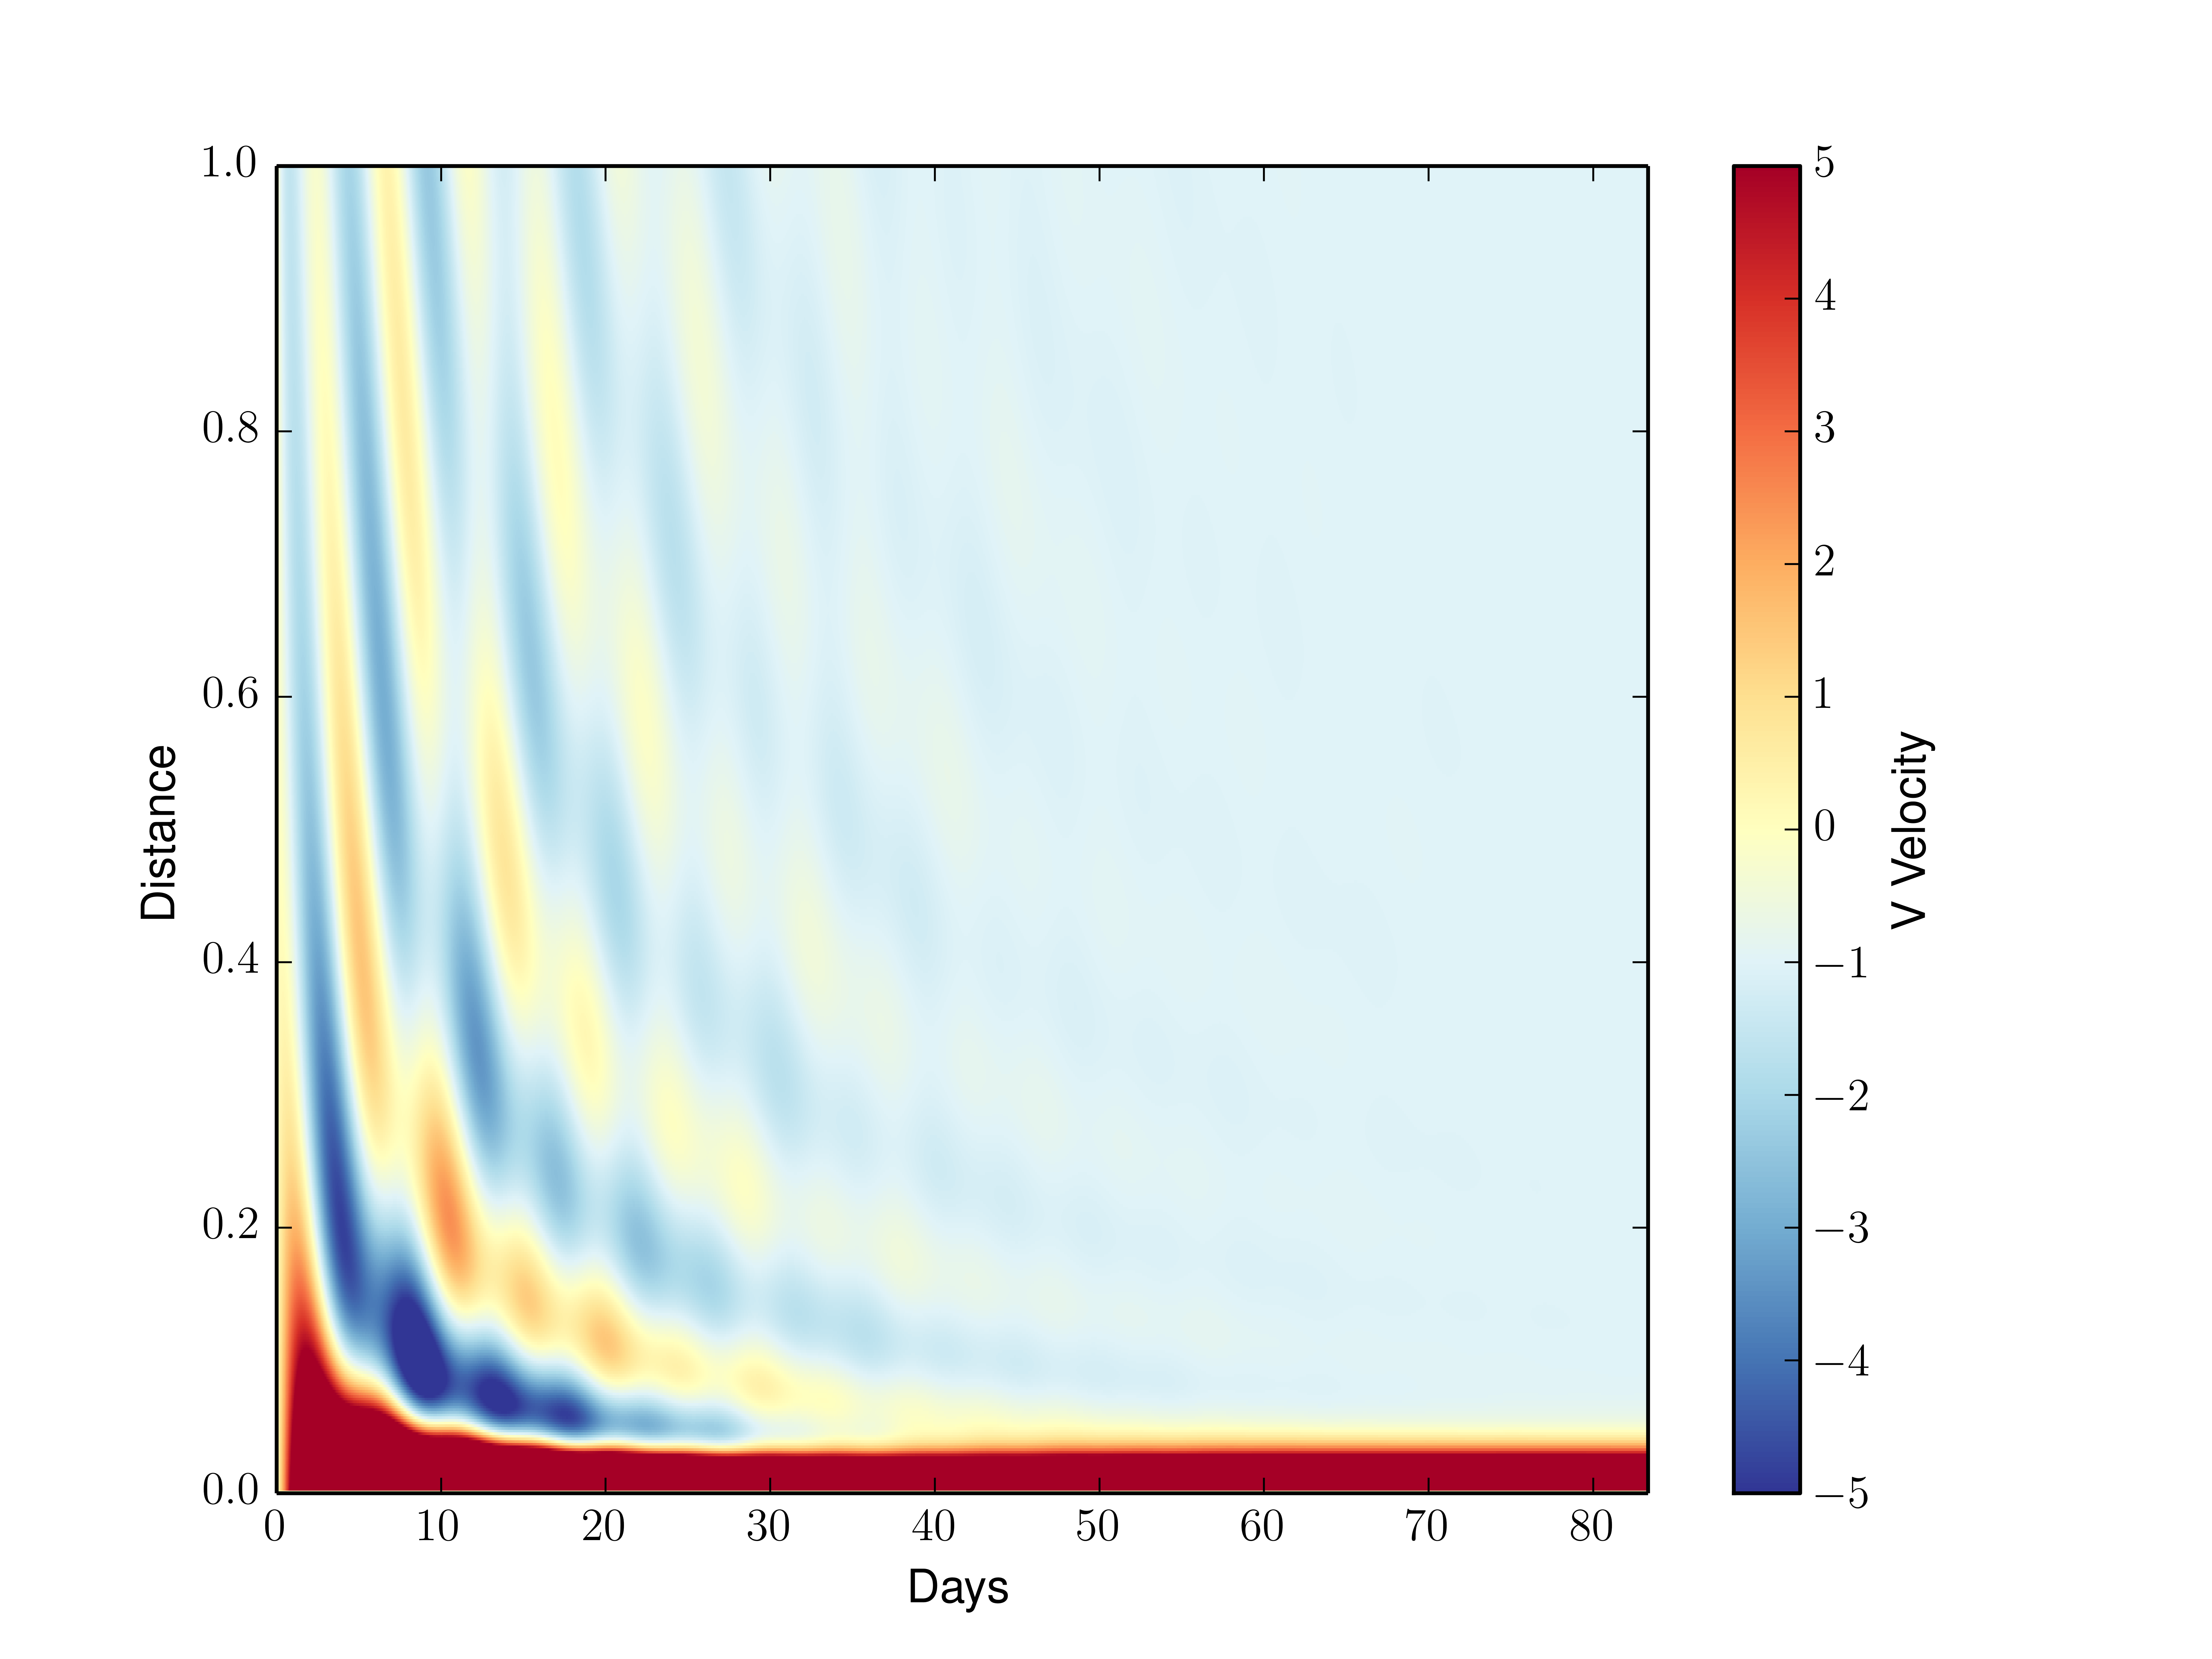
\includegraphics[width=6in]{../v_hovmuller.png}
\caption{Hovmuller Diagram of modeled velocity.}
\end{figure}

%% The Appendices part is started with the command \appendix;
%% appendix sections are then done as normal sections
%% \appendix

%% \section{}
%% \label{}

%% References
%%
%% Following citation commands can be used in the body text:
%% Usage of \cite is as follows:
%%   \cite{key}          ==>>  [#]
%%   \cite[chap. 2]{key} ==>>  [#, chap. 2]
%%   \citet{key}         ==>>  Author [#]

%% References with bibTeX database:

% \bibliographystyle{model1-num-names}
% \bibliography{sample.bib}

%% Authors are advised to submit their bibtex database files. They are
%% requested to list a bibtex style file in the manuscript if they do
%% not want to use model1-num-names.bst.

%% References without bibTeX database:

% \begin{thebibliography}{00}

%% \bibitem must have the following form:
%%   \bibitem{key}...
%%

% \bibitem{}

% \end{thebibliography}


\end{document}

%%
%% End of file `elsarticle-template-1-num.tex'.
              